\documentclass{standalone}
\usepackage{graphicx}	
\usepackage{amssymb, amsmath}
\usepackage{color}

\usepackage{tikz}
\usetikzlibrary{intersections, backgrounds}

\definecolor{light}{RGB}{220, 188, 188}
\definecolor{mid}{RGB}{185, 124, 124}
\definecolor{dark}{RGB}{143, 39, 39}
\definecolor{highlight}{RGB}{180, 31, 180}
\definecolor{gray10}{gray}{0.1}
\definecolor{gray20}{gray}{0.2}
\definecolor{gray30}{gray}{0.3}
\definecolor{gray40}{gray}{0.4}
\definecolor{gray60}{gray}{0.6}
\definecolor{gray70}{gray}{0.7}
\definecolor{gray80}{gray}{0.8}
\definecolor{gray90}{gray}{0.9}
\definecolor{gray95}{gray}{0.95}

\newcommand*{\offset}{0.025}

\begin{document}

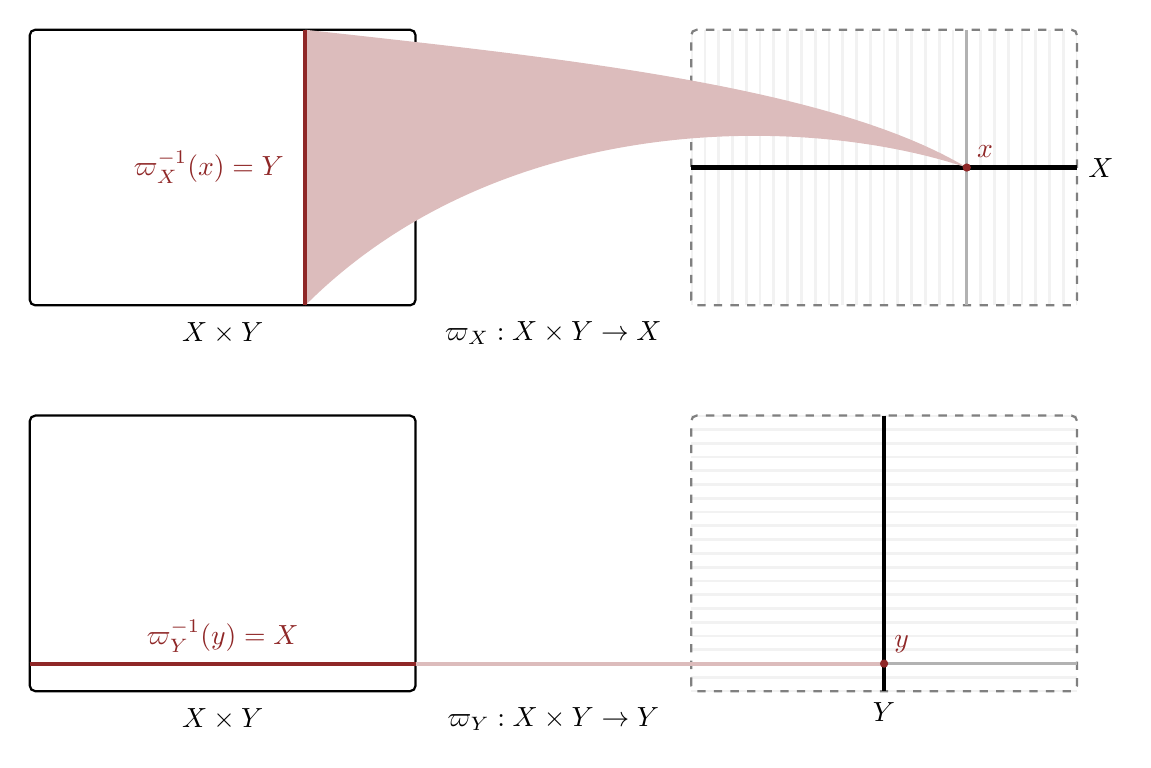
\begin{tikzpicture}[scale=0.35, thick]
  \draw [rounded corners=2pt, color=black] (-5, 0) rectangle +(-14, 10);
  \node at (-12, -1) { $X \times Y$ };

  \node at (0, -1) { $\varpi_{X}: X \times Y \rightarrow X$ };
  
  \begin{scope}
    \clip (5, 0) rectangle +(14, 10);
    \foreach \i in {5, 5.5, ..., 19} {
      \draw [color=gray95, line width=1] (\i, 0) -- +(0, 10);
    }  
  \end{scope}
  
  \draw [rounded corners=2pt, color=gray, dashed] (5, 0) rectangle +(14, 10);
  
  \draw [color=gray70, line width=1] (15, 0) -- +(0, 10);
  
  \draw [line width=1.5] (5, 5) -- +(14, 0)
  node[right] { $X$ };
  
  \fill [color=light] (-9, 0) -- (-9, 10) .. controls (0, 9) and (10, 8) .. (15, 5) 
                      .. controls (9, 7) and (-2, 7) .. (-9, 0);
  
  \fill [fill=dark, text=dark] (15, 5) circle (0.15)
  node[above right] { $x$ };
  
  \draw [color=dark, line width=1.5] (-9, 0) -- +(0, 10);
  \node[color=dark] at (-12.5, 5) {$\varpi_{X}^{-1}(x) = Y$};
  
  %
  
  \draw [rounded corners=2pt, color=black] (-5, -14) rectangle +(-14, 10);
  \node at (-12, -15) { $X \times Y$ };

  \node at (0, -15) { $\varpi_{Y}: X \times Y \rightarrow Y$ };
  
  \begin{scope}
    \clip (5, -14) rectangle +(14, 10);
    \foreach \i in {-14, -13.5, ..., -4} {
      \draw [color=gray95, line width=1] (5, \i) -- +(14, 0);
    }  
  \end{scope}
  
  \draw [rounded corners=2pt, color=gray, dashed] (5, -14) rectangle +(14, 10);
  
  \draw [color=gray70, line width=1] (5, -13) -- +(14, 0);
  
  \draw [line width=1.5] (12, -4) -- +(0, -10)
  node[below] { $Y$ };
  
  \draw [color=light, line width=1.5] (-19, -13) -- (12, -13);
  
  \fill [fill=dark, text=dark] (12, -13) circle (0.15)
  node[above right] { $y$ };
  
  \draw [color=dark, line width=1.5] (-5, -13) -- +(-14, 0);
  \node[color=dark] at (-12, -12) {$\varpi_{Y}^{-1}(y) = X$};
  
    
\end{tikzpicture}

\end{document}  